%*************************************************************************
% A Classic Thesis Style
% An Homage to The Elements of Typographic Style
%
% Copyright (C) 2017 André Miede and Ivo Pletikosić
%
% If you like the style then I would appreciate a postcard. My address
% can be found in the file ClassicThesis.pdf. A collection of the
% postcards I received so far is available online at
% http://postcards.miede.de
%
% License:
% This program is free software; you can redistribute it and/or modify
% it under the terms of the GNU General Public License as published by
% the Free Software Foundation; either version 2 of the License, or
% (at your option) any later version.
%
% This program is distributed in the hope that it will be useful,
% but WITHOUT ANY WARRANTY; without even the implied warranty of
% MERCHANTABILITY or FITNESS FOR A PARTICULAR PURPOSE.  See the
% GNU General Public License for more details.
    %
% You should have received a copy of the GNU General Public License
% along with this program; see the file COPYING.  If not, write to
% the Free Software Foundation, Inc., 59 Temple Place - Suite 330,
% Boston, MA 02111-1307, USA.
%
% PLEASE SEE ALSO THE AUTHORS' NOTE REGARDING THIS LICENSE
% IN THE DOCUMENTATION (ClassicThesis.pdf --> Chapter 1 / Chapter01.tex)
%*************************************************************************
\RequirePackage{silence} % :-\
    \WarningFilter{scrreprt}{Usage of package `titlesec'}
    %\WarningFilter{scrreprt}{Activating an ugly workaround}
    \WarningFilter{titlesec}{Non standard sectioning command detected}
\documentclass[ openright,titlepage,numbers=noenddot,headinclude,%twoside, %1headlines,% letterpaper a4paper
                footinclude=true,cleardoublepage=empty,abstractoff, % <--- obsolete, remove (todo)
                BCOR=5mm,paper=a4,fontsize=11pt,%11pt,a4paper,%
                ngerman,american,%lockflag%
                ]{scrreprt}

%*************************************************************************
% Note: Make all your adjustments in here
%*************************************************************************
% ****************************************************************************************************
% hdathesis-config.tex 
% Use it at the beginning of your thesis.tex, or as a LaTeX Preamble 
% in your thesis.{tex,lyx} with % ****************************************************************************************************
% hdathesis-config.tex 
% Use it at the beginning of your thesis.tex, or as a LaTeX Preamble 
% in your thesis.{tex,lyx} with % ****************************************************************************************************
% hdathesis-config.tex 
% Use it at the beginning of your thesis.tex, or as a LaTeX Preamble 
% in your thesis.{tex,lyx} with \input{hdathesis-config}
% ****************************************************************************************************

% ****************************************************************************************************
% 1. Personal data and user ad-hoc commands
% ****************************************************************************************************
\newcommand{\myTitle}{Database solution for the energy cluster application\xspace}
%\newcommand{\mySubtitle}{An Homage to The Elements of Typographic Style\xspace}
\newcommand{\myDegree}{Bachelor of Science (B.Sc.)\xspace} 
%\newcommand{\myDegree}{Bachelor of Arts (B.A.)\xspace}
%\newcommand{\myDegree}{Master of Science (M.Sc.)\xspace}
%\newcommand{\myDegree}{Master of Arts (M.A.)\xspace}
\newcommand{\myName}{Piotr Jurek\xspace}
%\newcommand{\myId}{081542\xspace}
\newcommand{\myProf}{dr inż. Anna Plichta\xspace}
%\newcommand{\myOtherProf}{Prof. Dr. Martin Stiemerling\xspace}
\newcommand{\myFaculty}{Faculty of Computer Science and Telecommunications\xspace}
\newcommand{\myUni}{Tadeusz Kościuszko University of Technology\xspace}
\newcommand{\myLocation}{Cracow\xspace}
\newcommand{\myTime}{04. January 2023\xspace}
\newcommand{\myVersion}{version 4.4\xspace}

% ****************************************************************************************************
% 2. Is it a master thesis?
% ****************************************************************************************************
%\PassOptionsToPackage{master}{hdahesis} % uncomment if this is a master thesis 

% ****************************************************************************************************
% 3. Does the thesis have a lock flag?
% ****************************************************************************************************
%\PassOptionsToPackage{lockflag}{hdathesis} % uncomment if this thesis has a lock flag 

% ****************************************************************************************************
% 4. Loading some handy packages
% ****************************************************************************************************
% ****************************************************************************************************
% Packages with options that might require adjustments
% ****************************************************************************************************

%\PassOptionsToPackage{ngerman,american}{babel}   % change this to your language(s)
% Spanish languages need extra options in order to work with this template
%\PassOptionsToPackage{spanish,es-lcroman}{babel}
\usepackage{babel}


% ****************************************************************************************************

% ****************************************************************************************************
% 1. Personal data and user ad-hoc commands
% ****************************************************************************************************
\newcommand{\myTitle}{Database solution for the energy cluster application\xspace}
%\newcommand{\mySubtitle}{An Homage to The Elements of Typographic Style\xspace}
\newcommand{\myDegree}{Bachelor of Science (B.Sc.)\xspace} 
%\newcommand{\myDegree}{Bachelor of Arts (B.A.)\xspace}
%\newcommand{\myDegree}{Master of Science (M.Sc.)\xspace}
%\newcommand{\myDegree}{Master of Arts (M.A.)\xspace}
\newcommand{\myName}{Piotr Jurek\xspace}
%\newcommand{\myId}{081542\xspace}
\newcommand{\myProf}{dr inż. Anna Plichta\xspace}
%\newcommand{\myOtherProf}{Prof. Dr. Martin Stiemerling\xspace}
\newcommand{\myFaculty}{Faculty of Computer Science and Telecommunications\xspace}
\newcommand{\myUni}{Tadeusz Kościuszko University of Technology\xspace}
\newcommand{\myLocation}{Cracow\xspace}
\newcommand{\myTime}{04. January 2023\xspace}
\newcommand{\myVersion}{version 4.4\xspace}

% ****************************************************************************************************
% 2. Is it a master thesis?
% ****************************************************************************************************
%\PassOptionsToPackage{master}{hdahesis} % uncomment if this is a master thesis 

% ****************************************************************************************************
% 3. Does the thesis have a lock flag?
% ****************************************************************************************************
%\PassOptionsToPackage{lockflag}{hdathesis} % uncomment if this thesis has a lock flag 

% ****************************************************************************************************
% 4. Loading some handy packages
% ****************************************************************************************************
% ****************************************************************************************************
% Packages with options that might require adjustments
% ****************************************************************************************************

%\PassOptionsToPackage{ngerman,american}{babel}   % change this to your language(s)
% Spanish languages need extra options in order to work with this template
%\PassOptionsToPackage{spanish,es-lcroman}{babel}
\usepackage{babel}


% ****************************************************************************************************

% ****************************************************************************************************
% 1. Personal data and user ad-hoc commands
% ****************************************************************************************************
\newcommand{\myTitle}{Database solution for the energy cluster application\xspace}
%\newcommand{\mySubtitle}{An Homage to The Elements of Typographic Style\xspace}
\newcommand{\myDegree}{Bachelor of Science (B.Sc.)\xspace} 
%\newcommand{\myDegree}{Bachelor of Arts (B.A.)\xspace}
%\newcommand{\myDegree}{Master of Science (M.Sc.)\xspace}
%\newcommand{\myDegree}{Master of Arts (M.A.)\xspace}
\newcommand{\myName}{Piotr Jurek\xspace}
%\newcommand{\myId}{081542\xspace}
\newcommand{\myProf}{dr inż. Anna Plichta\xspace}
%\newcommand{\myOtherProf}{Prof. Dr. Martin Stiemerling\xspace}
\newcommand{\myFaculty}{Faculty of Computer Science and Telecommunications\xspace}
\newcommand{\myUni}{Tadeusz Kościuszko University of Technology\xspace}
\newcommand{\myLocation}{Cracow\xspace}
\newcommand{\myTime}{04. January 2023\xspace}
\newcommand{\myVersion}{version 4.4\xspace}

% ****************************************************************************************************
% 2. Is it a master thesis?
% ****************************************************************************************************
%\PassOptionsToPackage{master}{hdahesis} % uncomment if this is a master thesis 

% ****************************************************************************************************
% 3. Does the thesis have a lock flag?
% ****************************************************************************************************
%\PassOptionsToPackage{lockflag}{hdathesis} % uncomment if this thesis has a lock flag 

% ****************************************************************************************************
% 4. Loading some handy packages
% ****************************************************************************************************
% ****************************************************************************************************
% Packages with options that might require adjustments
% ****************************************************************************************************

%\PassOptionsToPackage{ngerman,american}{babel}   % change this to your language(s)
% Spanish languages need extra options in order to work with this template
%\PassOptionsToPackage{spanish,es-lcroman}{babel}
\usepackage{babel}


% ****************************************************************************************************
% classicthesis-config.tex
% formerly known as loadpackages.sty, classicthesis-ldpkg.sty, and classicthesis-preamble.sty
% Use it at the beginning of your ClassicThesis.tex, or as a LaTeX Preamble
% in your ClassicThesis.{tex,lyx} with % ****************************************************************************************************
% classicthesis-config.tex
% formerly known as loadpackages.sty, classicthesis-ldpkg.sty, and classicthesis-preamble.sty
% Use it at the beginning of your ClassicThesis.tex, or as a LaTeX Preamble
% in your ClassicThesis.{tex,lyx} with % ****************************************************************************************************
% classicthesis-config.tex
% formerly known as loadpackages.sty, classicthesis-ldpkg.sty, and classicthesis-preamble.sty
% Use it at the beginning of your ClassicThesis.tex, or as a LaTeX Preamble
% in your ClassicThesis.{tex,lyx} with \input{classicthesis-config}
% ****************************************************************************************************
% If you like the classicthesis, then I would appreciate a postcard.
% My address can be found in the file ClassicThesis.pdf. A collection
% of the postcards I received so far is available online at
% http://postcards.miede.de
% ****************************************************************************************************


% ****************************************************************************************************
% 0. Set the encoding of your files. UTF-8 is the only sensible encoding nowadays. If you can't read
% äöüßáéçèê∂åëæƒÏ€ then change the encoding setting in your editor, not the line below. If your editor
% does not support utf8 use another editor!
% ****************************************************************************************************
\PassOptionsToPackage{utf8}{inputenc}
  \usepackage{inputenc}

% ****************************************************************************************************
% 1. Configure classicthesis for your needs here, e.g., remove "drafting" below
% in order to deactivate the time-stamp on the pages
% (see ClassicThesis.pdf for more information):
% ****************************************************************************************************
\PassOptionsToPackage{
  drafting=false,   % print version information on the bottom of the pages
  tocaligned=false, % the left column of the toc will be aligned (no indentation)
  dottedtoc=true,   % page numbers in ToC flushed right
  parts=true,       % use part division
  eulerchapternumbers=true, % use AMS Euler for chapter font (otherwise Palatino)
  linedheaders=false,       % chaper headers will have line above and beneath
  floatperchapter=true,     % numbering per chapter for all floats (i.e., Figure 1.1)
  listings=true,    % load listings package and setup LoL
  subfig=true,      % setup for preloaded subfig package
  eulermath=false,  % use awesome Euler fonts for mathematical formulae (only with pdfLaTeX)
  beramono=true,    % toggle a nice monospaced font (w/ bold)
  minionpro=false   % setup for minion pro font; use minion pro small caps as well (only with pdfLaTeX)
}{classicthesis}


% ****************************************************************************************************
% 2. Personal data and user ad-hoc commands
% ****************************************************************************************************
%\newcommand{\myTitle}{A Classic Thesis Style\xspace}
%\newcommand{\mySubtitle}{An Homage to The Elements of Typographic Style\xspace}
%\newcommand{\myDegree}{Doktor-Ingenieur (Dr.-Ing.)\xspace}
%\newcommand{\myName}{André Miede\xspace}
%\newcommand{\myProf}{Put name here\xspace}
%\newcommand{\myOtherProf}{Put name here\xspace}
%\newcommand{\mySupervisor}{Put name here\xspace}
%\newcommand{\myFaculty}{Put data here\xspace}
%\newcommand{\myDepartment}{Put data here\xspace}
%\newcommand{\myUni}{Put data here\xspace}
%\newcommand{\myLocation}{Saarbrücken\xspace}
%\newcommand{\myTime}{October 2017\xspace}
%\newcommand{\myVersion}{version 4.4}

% ********************************************************************
% Setup, finetuning, and useful commands
% ********************************************************************
\newcounter{dummy} % necessary for correct hyperlinks (to index, bib, etc.)
\newlength{\abcd} % for ab..z string length calculation
\providecommand{\mLyX}{L\kern-.1667em\lower.25em\hbox{Y}\kern-.125emX\@}
\newcommand{\ie}{i.\,e.}
\newcommand{\Ie}{I.\,e.}
\newcommand{\eg}{e.\,g.}
\newcommand{\Eg}{E.\,g.}
% ****************************************************************************************************


% ****************************************************************************************************
% 3. Loading some handy packages
% ****************************************************************************************************
% ********************************************************************
% Packages with options that might require adjustments
% ********************************************************************
%\PassOptionsToPackage{ngerman,american}{babel}   % change this to your language(s), main language last
% Spanish languages need extra options in order to work with this template
%\PassOptionsToPackage{spanish,es-lcroman}{babel}
\usepackage{babel}

\usepackage{csquotes}

\PassOptionsToPackage{%
  %backend=biber,bibencoding=utf8, %instead of bibtex
  backend=bibtex8,bibencoding=ascii,%
  language=auto,%
  %style=numeric-comp,%
  style=alphabetic,%
  %style=authoryear-comp, % Author 1999, 2010
  %bibstyle=authoryear,dashed=false, % dashed: substitute rep. author with ---
  sorting=nyt, % name, year, title
  maxbibnames=10, % default: 3, et al.
  %backref=true,%
  natbib=true % natbib compatibility mode (\citep and \citet still work)
}{biblatex}
  \usepackage{biblatex}

\PassOptionsToPackage{fleqn}{amsmath}       % math environments and more by the AMS
  \usepackage{amsmath}

\PassOptionsToPackage{doublespacing}{hdathesis}  % options: abbrev exam big wiwi english master
  \usepackage{hdathesis}

% ********************************************************************
% General useful packages
% ********************************************************************
\PassOptionsToPackage{T1}{fontenc} % T2A for cyrillics
  \usepackage{fontenc}
\usepackage{textcomp} % fix warning with missing font shapes
\usepackage{scrhack} % fix warnings when using KOMA with listings package
\usepackage{xspace} % to get the spacing after macros right
\usepackage{mparhack} % get marginpar right
%\usepackage{fixltx2e} % fixes some LaTeX stuff --> since 2015 in the LaTeX kernel (see below)
% \usepackage[latest]{latexrelease} % emulate newer kernel version if older is detected
\PassOptionsToPackage{printonlyused,smaller}{acronym}
  \usepackage{acronym} % nice macros for handling all acronyms in the thesis
  %\renewcommand{\bflabel}[1]{{#1}\hfill} % fix the list of acronyms --> no longer working
  %\renewcommand*{\acsfont}[1]{\textsc{#1}}
  %\renewcommand*{\aclabelfont}[1]{\acsfont{#1}}
  %\def\bflabel#1{{#1\hfill}}
  \def\bflabel#1{{\acsfont{#1}\hfill}}
  \def\aclabelfont#1{\acsfont{#1}}
% ****************************************************************************************************
%\usepackage{pgfplots} % External TikZ/PGF support (thanks to Andreas Nautsch)
%\usetikzlibrary{external}
%\tikzexternalize[mode=list and make, prefix=ext-tikz/]
% ****************************************************************************************************


% ****************************************************************************************************
% 4. Setup floats: tables, (sub)figures, and captions
% ****************************************************************************************************
\usepackage{tabularx} % better tables
  \setlength{\extrarowheight}{3pt} % increase table row height
\newcommand{\tableheadline}[1]{\multicolumn{1}{c}{\spacedlowsmallcaps{#1}}}
\newcommand{\myfloatalign}{\centering} % to be used with each float for alignment
\usepackage{caption}
% Thanks to cgnieder and Claus Lahiri
% http://tex.stackexchange.com/questions/69349/spacedlowsmallcaps-in-caption-label
% [REMOVED DUE TO OTHER PROBLEMS, SEE ISSUE #82]
%\DeclareCaptionLabelFormat{smallcaps}{\bothIfFirst{#1}{~}\MakeTextLowercase{\textsc{#2}}}
%\captionsetup{font=small,labelformat=smallcaps} % format=hang,
\captionsetup{font=small} % format=hang,
\usepackage{subfig}
% ****************************************************************************************************


% ****************************************************************************************************
% 5. Setup code listings
% ****************************************************************************************************
\usepackage{listings}
%\lstset{emph={trueIndex,root},emphstyle=\color{BlueViolet}}%\underbar} % for special keywords
\lstset{language=[LaTeX]Tex,%C++,
  morekeywords={PassOptionsToPackage,selectlanguage},
  keywordstyle=\color{RoyalBlue},%\bfseries,
  basicstyle=\small\ttfamily,
  %identifierstyle=\color{NavyBlue},
  commentstyle=\color{Green}\ttfamily,
  stringstyle=\rmfamily,
  numbers=none,%left,%
  numberstyle=\scriptsize,%\tiny
  stepnumber=5,
  numbersep=8pt,
  showstringspaces=false,
  breaklines=true,
  %frameround=ftff,
  %frame=single,
  belowcaptionskip=.75\baselineskip
  %frame=L
}
% ****************************************************************************************************


% ****************************************************************************************************
% 6. PDFLaTeX, hyperreferences, and citation backreferences
% ****************************************************************************************************
% ********************************************************************
% Using PDFLaTeX
% ********************************************************************
\PassOptionsToPackage{hyperfootnotes=false,pdfpagelabels}{hyperref}
  \usepackage{hyperref}  % backref linktocpage pagebackref
%\ifpdf
%\pdfcompresslevel=9
%\pdfadjustspacing=1
%\fi
%\PassOptionsToPackage{pdftex}{graphicx} %%%IVO: driver will be chosen automatically
  \usepackage{graphicx}


% ********************************************************************
% Hyperreferences
% ********************************************************************
\hypersetup{%
  %draft, % hyperref's draft mode, for printing see below
  colorlinks=true, linktocpage=true, pdfstartpage=3, pdfstartview=FitV,%
  % uncomment the following line if you want to have black links (e.g., for printing)
  %colorlinks=false, linktocpage=false, pdfstartpage=3, pdfstartview=FitV, pdfborder={0 0 0},%
  breaklinks=true, pdfpagemode=UseNone, pageanchor=true, pdfpagemode=UseOutlines,%
  plainpages=false, bookmarksnumbered, bookmarksopen=true, bookmarksopenlevel=1,%
  hypertexnames=true, pdfhighlight=/O,%nesting=true,%frenchlinks,%
  urlcolor=webbrown, linkcolor=RoyalBlue, citecolor=webgreen, %pagecolor=RoyalBlue,%
  %urlcolor=Black, linkcolor=Black, citecolor=Black, %pagecolor=Black,%
  pdftitle={\myTitle},%
  pdfauthor={\textcopyright\ \myName, \myUni, \myFaculty},%
  pdfsubject={},%
  pdfkeywords={},%
  pdfcreator={pdfLaTeX},%
  pdfproducer={LaTeX with hyperref and classicthesis}%
}

% ********************************************************************
% Setup autoreferences
% ********************************************************************
% There are some issues regarding autorefnames
% http://www.ureader.de/msg/136221647.aspx
% http://www.tex.ac.uk/cgi-bin/texfaq2html?label=latexwords
% you have to redefine the makros for the
% language you use, e.g., american, ngerman
% (as chosen when loading babel/AtBeginDocument)
% ********************************************************************
\makeatletter
\@ifpackageloaded{babel}%
  {%
    \addto\extrasamerican{%
      \renewcommand*{\figureautorefname}{Figure}%
      \renewcommand*{\tableautorefname}{Table}%
      \renewcommand*{\partautorefname}{Part}%
      \renewcommand*{\chapterautorefname}{Chapter}%
      \renewcommand*{\sectionautorefname}{Section}%
      \renewcommand*{\subsectionautorefname}{Section}%
      \renewcommand*{\subsubsectionautorefname}{Section}%
    }%
    \addto\extrasngerman{%
      \renewcommand*{\paragraphautorefname}{Absatz}%
      \renewcommand*{\subparagraphautorefname}{Unterabsatz}%
      \renewcommand*{\footnoteautorefname}{Fu\"snote}%
      \renewcommand*{\FancyVerbLineautorefname}{Zeile}%
      \renewcommand*{\theoremautorefname}{Theorem}%
      \renewcommand*{\appendixautorefname}{Anhang}%
      \renewcommand*{\equationautorefname}{Gleichung}%
      \renewcommand*{\itemautorefname}{Punkt}%
    }%
      % Fix to getting autorefs for subfigures right (thanks to Belinda Vogt for changing the definition)
      \providecommand{\subfigureautorefname}{\figureautorefname}%
    }{\relax}
\makeatother


% ****************************************************************************************************
% 7. Last calls before the bar closes
% ****************************************************************************************************
% ********************************************************************
% Development Stuff
% ********************************************************************
\listfiles
%\PassOptionsToPackage{l2tabu,orthodox,abort}{nag}
%  \usepackage{nag}
%\PassOptionsToPackage{warning, all}{onlyamsmath}
%  \usepackage{onlyamsmath}

% ********************************************************************
% Last, but not least...
% ********************************************************************
\usepackage{classicthesis}
% ****************************************************************************************************


% ****************************************************************************************************
% 8. Further adjustments (experimental)
% ****************************************************************************************************
% ********************************************************************
% Changing the text area
% ********************************************************************
\areaset[current]{312pt}{821pt} % 686 (factor 2.2) + 33 head + 42 head \the\footskip
%\setlength{\marginparwidth}{7em}%
%\setlength{\marginparsep}{2em}%

% ********************************************************************
% Using different fonts
% ********************************************************************
%\usepackage[oldstylenums]{kpfonts} % oldstyle notextcomp
%\usepackage[osf]{libertine}
%\usepackage[light,condensed,math]{iwona}
%\renewcommand{\sfdefault}{iwona}
%\usepackage{lmodern} % <-- no osf support :-(
%\usepackage{cfr-lm} %
%\usepackage[urw-garamond]{mathdesign} <-- no osf support :-(
%\usepackage[default,osfigures]{opensans} % scale=0.95
%\usepackage[sfdefault]{FiraSans}
% ********************************************************************
% \usepackage[largesc,osf]{newpxtext}
% Used to fix these:
% https://bitbucket.org/amiede/classicthesis/issues/139/italics-in-pallatino-capitals-chapter
% https://bitbucket.org/amiede/classicthesis/issues/45/problema-testatine-su-classicthesis-style
% ********************************************************************
%\linespread{1.05} % a bit more for Palatino
% ****************************************************************************************************

% ****************************************************************************************************
% If you like the classicthesis, then I would appreciate a postcard.
% My address can be found in the file ClassicThesis.pdf. A collection
% of the postcards I received so far is available online at
% http://postcards.miede.de
% ****************************************************************************************************


% ****************************************************************************************************
% 0. Set the encoding of your files. UTF-8 is the only sensible encoding nowadays. If you can't read
% äöüßáéçèê∂åëæƒÏ€ then change the encoding setting in your editor, not the line below. If your editor
% does not support utf8 use another editor!
% ****************************************************************************************************
\PassOptionsToPackage{utf8}{inputenc}
  \usepackage{inputenc}

% ****************************************************************************************************
% 1. Configure classicthesis for your needs here, e.g., remove "drafting" below
% in order to deactivate the time-stamp on the pages
% (see ClassicThesis.pdf for more information):
% ****************************************************************************************************
\PassOptionsToPackage{
  drafting=false,   % print version information on the bottom of the pages
  tocaligned=false, % the left column of the toc will be aligned (no indentation)
  dottedtoc=true,   % page numbers in ToC flushed right
  parts=true,       % use part division
  eulerchapternumbers=true, % use AMS Euler for chapter font (otherwise Palatino)
  linedheaders=false,       % chaper headers will have line above and beneath
  floatperchapter=true,     % numbering per chapter for all floats (i.e., Figure 1.1)
  listings=true,    % load listings package and setup LoL
  subfig=true,      % setup for preloaded subfig package
  eulermath=false,  % use awesome Euler fonts for mathematical formulae (only with pdfLaTeX)
  beramono=true,    % toggle a nice monospaced font (w/ bold)
  minionpro=false   % setup for minion pro font; use minion pro small caps as well (only with pdfLaTeX)
}{classicthesis}


% ****************************************************************************************************
% 2. Personal data and user ad-hoc commands
% ****************************************************************************************************
%\newcommand{\myTitle}{A Classic Thesis Style\xspace}
%\newcommand{\mySubtitle}{An Homage to The Elements of Typographic Style\xspace}
%\newcommand{\myDegree}{Doktor-Ingenieur (Dr.-Ing.)\xspace}
%\newcommand{\myName}{André Miede\xspace}
%\newcommand{\myProf}{Put name here\xspace}
%\newcommand{\myOtherProf}{Put name here\xspace}
%\newcommand{\mySupervisor}{Put name here\xspace}
%\newcommand{\myFaculty}{Put data here\xspace}
%\newcommand{\myDepartment}{Put data here\xspace}
%\newcommand{\myUni}{Put data here\xspace}
%\newcommand{\myLocation}{Saarbrücken\xspace}
%\newcommand{\myTime}{October 2017\xspace}
%\newcommand{\myVersion}{version 4.4}

% ********************************************************************
% Setup, finetuning, and useful commands
% ********************************************************************
\newcounter{dummy} % necessary for correct hyperlinks (to index, bib, etc.)
\newlength{\abcd} % for ab..z string length calculation
\providecommand{\mLyX}{L\kern-.1667em\lower.25em\hbox{Y}\kern-.125emX\@}
\newcommand{\ie}{i.\,e.}
\newcommand{\Ie}{I.\,e.}
\newcommand{\eg}{e.\,g.}
\newcommand{\Eg}{E.\,g.}
% ****************************************************************************************************


% ****************************************************************************************************
% 3. Loading some handy packages
% ****************************************************************************************************
% ********************************************************************
% Packages with options that might require adjustments
% ********************************************************************
%\PassOptionsToPackage{ngerman,american}{babel}   % change this to your language(s), main language last
% Spanish languages need extra options in order to work with this template
%\PassOptionsToPackage{spanish,es-lcroman}{babel}
\usepackage{babel}

\usepackage{csquotes}

\PassOptionsToPackage{%
  %backend=biber,bibencoding=utf8, %instead of bibtex
  backend=bibtex8,bibencoding=ascii,%
  language=auto,%
  %style=numeric-comp,%
  style=alphabetic,%
  %style=authoryear-comp, % Author 1999, 2010
  %bibstyle=authoryear,dashed=false, % dashed: substitute rep. author with ---
  sorting=nyt, % name, year, title
  maxbibnames=10, % default: 3, et al.
  %backref=true,%
  natbib=true % natbib compatibility mode (\citep and \citet still work)
}{biblatex}
  \usepackage{biblatex}

\PassOptionsToPackage{fleqn}{amsmath}       % math environments and more by the AMS
  \usepackage{amsmath}

\PassOptionsToPackage{doublespacing}{hdathesis}  % options: abbrev exam big wiwi english master
  \usepackage{hdathesis}

% ********************************************************************
% General useful packages
% ********************************************************************
\PassOptionsToPackage{T1}{fontenc} % T2A for cyrillics
  \usepackage{fontenc}
\usepackage{textcomp} % fix warning with missing font shapes
\usepackage{scrhack} % fix warnings when using KOMA with listings package
\usepackage{xspace} % to get the spacing after macros right
\usepackage{mparhack} % get marginpar right
%\usepackage{fixltx2e} % fixes some LaTeX stuff --> since 2015 in the LaTeX kernel (see below)
% \usepackage[latest]{latexrelease} % emulate newer kernel version if older is detected
\PassOptionsToPackage{printonlyused,smaller}{acronym}
  \usepackage{acronym} % nice macros for handling all acronyms in the thesis
  %\renewcommand{\bflabel}[1]{{#1}\hfill} % fix the list of acronyms --> no longer working
  %\renewcommand*{\acsfont}[1]{\textsc{#1}}
  %\renewcommand*{\aclabelfont}[1]{\acsfont{#1}}
  %\def\bflabel#1{{#1\hfill}}
  \def\bflabel#1{{\acsfont{#1}\hfill}}
  \def\aclabelfont#1{\acsfont{#1}}
% ****************************************************************************************************
%\usepackage{pgfplots} % External TikZ/PGF support (thanks to Andreas Nautsch)
%\usetikzlibrary{external}
%\tikzexternalize[mode=list and make, prefix=ext-tikz/]
% ****************************************************************************************************


% ****************************************************************************************************
% 4. Setup floats: tables, (sub)figures, and captions
% ****************************************************************************************************
\usepackage{tabularx} % better tables
  \setlength{\extrarowheight}{3pt} % increase table row height
\newcommand{\tableheadline}[1]{\multicolumn{1}{c}{\spacedlowsmallcaps{#1}}}
\newcommand{\myfloatalign}{\centering} % to be used with each float for alignment
\usepackage{caption}
% Thanks to cgnieder and Claus Lahiri
% http://tex.stackexchange.com/questions/69349/spacedlowsmallcaps-in-caption-label
% [REMOVED DUE TO OTHER PROBLEMS, SEE ISSUE #82]
%\DeclareCaptionLabelFormat{smallcaps}{\bothIfFirst{#1}{~}\MakeTextLowercase{\textsc{#2}}}
%\captionsetup{font=small,labelformat=smallcaps} % format=hang,
\captionsetup{font=small} % format=hang,
\usepackage{subfig}
% ****************************************************************************************************


% ****************************************************************************************************
% 5. Setup code listings
% ****************************************************************************************************
\usepackage{listings}
%\lstset{emph={trueIndex,root},emphstyle=\color{BlueViolet}}%\underbar} % for special keywords
\lstset{language=[LaTeX]Tex,%C++,
  morekeywords={PassOptionsToPackage,selectlanguage},
  keywordstyle=\color{RoyalBlue},%\bfseries,
  basicstyle=\small\ttfamily,
  %identifierstyle=\color{NavyBlue},
  commentstyle=\color{Green}\ttfamily,
  stringstyle=\rmfamily,
  numbers=none,%left,%
  numberstyle=\scriptsize,%\tiny
  stepnumber=5,
  numbersep=8pt,
  showstringspaces=false,
  breaklines=true,
  %frameround=ftff,
  %frame=single,
  belowcaptionskip=.75\baselineskip
  %frame=L
}
% ****************************************************************************************************


% ****************************************************************************************************
% 6. PDFLaTeX, hyperreferences, and citation backreferences
% ****************************************************************************************************
% ********************************************************************
% Using PDFLaTeX
% ********************************************************************
\PassOptionsToPackage{hyperfootnotes=false,pdfpagelabels}{hyperref}
  \usepackage{hyperref}  % backref linktocpage pagebackref
%\ifpdf
%\pdfcompresslevel=9
%\pdfadjustspacing=1
%\fi
%\PassOptionsToPackage{pdftex}{graphicx} %%%IVO: driver will be chosen automatically
  \usepackage{graphicx}


% ********************************************************************
% Hyperreferences
% ********************************************************************
\hypersetup{%
  %draft, % hyperref's draft mode, for printing see below
  colorlinks=true, linktocpage=true, pdfstartpage=3, pdfstartview=FitV,%
  % uncomment the following line if you want to have black links (e.g., for printing)
  %colorlinks=false, linktocpage=false, pdfstartpage=3, pdfstartview=FitV, pdfborder={0 0 0},%
  breaklinks=true, pdfpagemode=UseNone, pageanchor=true, pdfpagemode=UseOutlines,%
  plainpages=false, bookmarksnumbered, bookmarksopen=true, bookmarksopenlevel=1,%
  hypertexnames=true, pdfhighlight=/O,%nesting=true,%frenchlinks,%
  urlcolor=webbrown, linkcolor=RoyalBlue, citecolor=webgreen, %pagecolor=RoyalBlue,%
  %urlcolor=Black, linkcolor=Black, citecolor=Black, %pagecolor=Black,%
  pdftitle={\myTitle},%
  pdfauthor={\textcopyright\ \myName, \myUni, \myFaculty},%
  pdfsubject={},%
  pdfkeywords={},%
  pdfcreator={pdfLaTeX},%
  pdfproducer={LaTeX with hyperref and classicthesis}%
}

% ********************************************************************
% Setup autoreferences
% ********************************************************************
% There are some issues regarding autorefnames
% http://www.ureader.de/msg/136221647.aspx
% http://www.tex.ac.uk/cgi-bin/texfaq2html?label=latexwords
% you have to redefine the makros for the
% language you use, e.g., american, ngerman
% (as chosen when loading babel/AtBeginDocument)
% ********************************************************************
\makeatletter
\@ifpackageloaded{babel}%
  {%
    \addto\extrasamerican{%
      \renewcommand*{\figureautorefname}{Figure}%
      \renewcommand*{\tableautorefname}{Table}%
      \renewcommand*{\partautorefname}{Part}%
      \renewcommand*{\chapterautorefname}{Chapter}%
      \renewcommand*{\sectionautorefname}{Section}%
      \renewcommand*{\subsectionautorefname}{Section}%
      \renewcommand*{\subsubsectionautorefname}{Section}%
    }%
    \addto\extrasngerman{%
      \renewcommand*{\paragraphautorefname}{Absatz}%
      \renewcommand*{\subparagraphautorefname}{Unterabsatz}%
      \renewcommand*{\footnoteautorefname}{Fu\"snote}%
      \renewcommand*{\FancyVerbLineautorefname}{Zeile}%
      \renewcommand*{\theoremautorefname}{Theorem}%
      \renewcommand*{\appendixautorefname}{Anhang}%
      \renewcommand*{\equationautorefname}{Gleichung}%
      \renewcommand*{\itemautorefname}{Punkt}%
    }%
      % Fix to getting autorefs for subfigures right (thanks to Belinda Vogt for changing the definition)
      \providecommand{\subfigureautorefname}{\figureautorefname}%
    }{\relax}
\makeatother


% ****************************************************************************************************
% 7. Last calls before the bar closes
% ****************************************************************************************************
% ********************************************************************
% Development Stuff
% ********************************************************************
\listfiles
%\PassOptionsToPackage{l2tabu,orthodox,abort}{nag}
%  \usepackage{nag}
%\PassOptionsToPackage{warning, all}{onlyamsmath}
%  \usepackage{onlyamsmath}

% ********************************************************************
% Last, but not least...
% ********************************************************************
\usepackage{classicthesis}
% ****************************************************************************************************


% ****************************************************************************************************
% 8. Further adjustments (experimental)
% ****************************************************************************************************
% ********************************************************************
% Changing the text area
% ********************************************************************
\areaset[current]{312pt}{821pt} % 686 (factor 2.2) + 33 head + 42 head \the\footskip
%\setlength{\marginparwidth}{7em}%
%\setlength{\marginparsep}{2em}%

% ********************************************************************
% Using different fonts
% ********************************************************************
%\usepackage[oldstylenums]{kpfonts} % oldstyle notextcomp
%\usepackage[osf]{libertine}
%\usepackage[light,condensed,math]{iwona}
%\renewcommand{\sfdefault}{iwona}
%\usepackage{lmodern} % <-- no osf support :-(
%\usepackage{cfr-lm} %
%\usepackage[urw-garamond]{mathdesign} <-- no osf support :-(
%\usepackage[default,osfigures]{opensans} % scale=0.95
%\usepackage[sfdefault]{FiraSans}
% ********************************************************************
% \usepackage[largesc,osf]{newpxtext}
% Used to fix these:
% https://bitbucket.org/amiede/classicthesis/issues/139/italics-in-pallatino-capitals-chapter
% https://bitbucket.org/amiede/classicthesis/issues/45/problema-testatine-su-classicthesis-style
% ********************************************************************
%\linespread{1.05} % a bit more for Palatino
% ****************************************************************************************************

% ****************************************************************************************************
% If you like the classicthesis, then I would appreciate a postcard.
% My address can be found in the file ClassicThesis.pdf. A collection
% of the postcards I received so far is available online at
% http://postcards.miede.de
% ****************************************************************************************************


% ****************************************************************************************************
% 0. Set the encoding of your files. UTF-8 is the only sensible encoding nowadays. If you can't read
% äöüßáéçèê∂åëæƒÏ€ then change the encoding setting in your editor, not the line below. If your editor
% does not support utf8 use another editor!
% ****************************************************************************************************
\PassOptionsToPackage{utf8}{inputenc}
  \usepackage{inputenc}

% ****************************************************************************************************
% 1. Configure classicthesis for your needs here, e.g., remove "drafting" below
% in order to deactivate the time-stamp on the pages
% (see ClassicThesis.pdf for more information):
% ****************************************************************************************************
\PassOptionsToPackage{
  drafting=false,   % print version information on the bottom of the pages
  tocaligned=false, % the left column of the toc will be aligned (no indentation)
  dottedtoc=true,   % page numbers in ToC flushed right
  parts=true,       % use part division
  eulerchapternumbers=true, % use AMS Euler for chapter font (otherwise Palatino)
  linedheaders=false,       % chaper headers will have line above and beneath
  floatperchapter=true,     % numbering per chapter for all floats (i.e., Figure 1.1)
  listings=true,    % load listings package and setup LoL
  subfig=true,      % setup for preloaded subfig package
  eulermath=false,  % use awesome Euler fonts for mathematical formulae (only with pdfLaTeX)
  beramono=true,    % toggle a nice monospaced font (w/ bold)
  minionpro=false   % setup for minion pro font; use minion pro small caps as well (only with pdfLaTeX)
}{classicthesis}


% ****************************************************************************************************
% 2. Personal data and user ad-hoc commands
% ****************************************************************************************************
%\newcommand{\myTitle}{A Classic Thesis Style\xspace}
%\newcommand{\mySubtitle}{An Homage to The Elements of Typographic Style\xspace}
%\newcommand{\myDegree}{Doktor-Ingenieur (Dr.-Ing.)\xspace}
%\newcommand{\myName}{André Miede\xspace}
%\newcommand{\myProf}{Put name here\xspace}
%\newcommand{\myOtherProf}{Put name here\xspace}
%\newcommand{\mySupervisor}{Put name here\xspace}
%\newcommand{\myFaculty}{Put data here\xspace}
%\newcommand{\myDepartment}{Put data here\xspace}
%\newcommand{\myUni}{Put data here\xspace}
%\newcommand{\myLocation}{Saarbrücken\xspace}
%\newcommand{\myTime}{October 2017\xspace}
%\newcommand{\myVersion}{version 4.4}

% ********************************************************************
% Setup, finetuning, and useful commands
% ********************************************************************
\newcounter{dummy} % necessary for correct hyperlinks (to index, bib, etc.)
\newlength{\abcd} % for ab..z string length calculation
\providecommand{\mLyX}{L\kern-.1667em\lower.25em\hbox{Y}\kern-.125emX\@}
\newcommand{\ie}{i.\,e.}
\newcommand{\Ie}{I.\,e.}
\newcommand{\eg}{e.\,g.}
\newcommand{\Eg}{E.\,g.}
% ****************************************************************************************************


% ****************************************************************************************************
% 3. Loading some handy packages
% ****************************************************************************************************
% ********************************************************************
% Packages with options that might require adjustments
% ********************************************************************
%\PassOptionsToPackage{ngerman,american}{babel}   % change this to your language(s), main language last
% Spanish languages need extra options in order to work with this template
%\PassOptionsToPackage{spanish,es-lcroman}{babel}
\usepackage{babel}

\usepackage{csquotes}

\PassOptionsToPackage{%
  %backend=biber,bibencoding=utf8, %instead of bibtex
  backend=bibtex8,bibencoding=ascii,%
  language=auto,%
  %style=numeric-comp,%
  style=alphabetic,%
  %style=authoryear-comp, % Author 1999, 2010
  %bibstyle=authoryear,dashed=false, % dashed: substitute rep. author with ---
  sorting=nyt, % name, year, title
  maxbibnames=10, % default: 3, et al.
  %backref=true,%
  natbib=true % natbib compatibility mode (\citep and \citet still work)
}{biblatex}
  \usepackage{biblatex}

\PassOptionsToPackage{fleqn}{amsmath}       % math environments and more by the AMS
  \usepackage{amsmath}

\PassOptionsToPackage{doublespacing}{hdathesis}  % options: abbrev exam big wiwi english master
  \usepackage{hdathesis}

% ********************************************************************
% General useful packages
% ********************************************************************
\PassOptionsToPackage{T1}{fontenc} % T2A for cyrillics
  \usepackage{fontenc}
\usepackage{textcomp} % fix warning with missing font shapes
\usepackage{scrhack} % fix warnings when using KOMA with listings package
\usepackage{xspace} % to get the spacing after macros right
\usepackage{mparhack} % get marginpar right
%\usepackage{fixltx2e} % fixes some LaTeX stuff --> since 2015 in the LaTeX kernel (see below)
% \usepackage[latest]{latexrelease} % emulate newer kernel version if older is detected
\PassOptionsToPackage{printonlyused,smaller}{acronym}
  \usepackage{acronym} % nice macros for handling all acronyms in the thesis
  %\renewcommand{\bflabel}[1]{{#1}\hfill} % fix the list of acronyms --> no longer working
  %\renewcommand*{\acsfont}[1]{\textsc{#1}}
  %\renewcommand*{\aclabelfont}[1]{\acsfont{#1}}
  %\def\bflabel#1{{#1\hfill}}
  \def\bflabel#1{{\acsfont{#1}\hfill}}
  \def\aclabelfont#1{\acsfont{#1}}
% ****************************************************************************************************
%\usepackage{pgfplots} % External TikZ/PGF support (thanks to Andreas Nautsch)
%\usetikzlibrary{external}
%\tikzexternalize[mode=list and make, prefix=ext-tikz/]
% ****************************************************************************************************


% ****************************************************************************************************
% 4. Setup floats: tables, (sub)figures, and captions
% ****************************************************************************************************
\usepackage{tabularx} % better tables
  \setlength{\extrarowheight}{3pt} % increase table row height
\newcommand{\tableheadline}[1]{\multicolumn{1}{c}{\spacedlowsmallcaps{#1}}}
\newcommand{\myfloatalign}{\centering} % to be used with each float for alignment
\usepackage{caption}
% Thanks to cgnieder and Claus Lahiri
% http://tex.stackexchange.com/questions/69349/spacedlowsmallcaps-in-caption-label
% [REMOVED DUE TO OTHER PROBLEMS, SEE ISSUE #82]
%\DeclareCaptionLabelFormat{smallcaps}{\bothIfFirst{#1}{~}\MakeTextLowercase{\textsc{#2}}}
%\captionsetup{font=small,labelformat=smallcaps} % format=hang,
\captionsetup{font=small} % format=hang,
\usepackage{subfig}
% ****************************************************************************************************


% ****************************************************************************************************
% 5. Setup code listings
% ****************************************************************************************************
\usepackage{listings}
%\lstset{emph={trueIndex,root},emphstyle=\color{BlueViolet}}%\underbar} % for special keywords
\lstset{language=[LaTeX]Tex,%C++,
  morekeywords={PassOptionsToPackage,selectlanguage},
  keywordstyle=\color{RoyalBlue},%\bfseries,
  basicstyle=\small\ttfamily,
  %identifierstyle=\color{NavyBlue},
  commentstyle=\color{Green}\ttfamily,
  stringstyle=\rmfamily,
  numbers=none,%left,%
  numberstyle=\scriptsize,%\tiny
  stepnumber=5,
  numbersep=8pt,
  showstringspaces=false,
  breaklines=true,
  %frameround=ftff,
  %frame=single,
  belowcaptionskip=.75\baselineskip
  %frame=L
}
% ****************************************************************************************************


% ****************************************************************************************************
% 6. PDFLaTeX, hyperreferences, and citation backreferences
% ****************************************************************************************************
% ********************************************************************
% Using PDFLaTeX
% ********************************************************************
\PassOptionsToPackage{hyperfootnotes=false,pdfpagelabels}{hyperref}
  \usepackage{hyperref}  % backref linktocpage pagebackref
%\ifpdf
%\pdfcompresslevel=9
%\pdfadjustspacing=1
%\fi
%\PassOptionsToPackage{pdftex}{graphicx} %%%IVO: driver will be chosen automatically
  \usepackage{graphicx}


% ********************************************************************
% Hyperreferences
% ********************************************************************
\hypersetup{%
  %draft, % hyperref's draft mode, for printing see below
  colorlinks=true, linktocpage=true, pdfstartpage=3, pdfstartview=FitV,%
  % uncomment the following line if you want to have black links (e.g., for printing)
  %colorlinks=false, linktocpage=false, pdfstartpage=3, pdfstartview=FitV, pdfborder={0 0 0},%
  breaklinks=true, pdfpagemode=UseNone, pageanchor=true, pdfpagemode=UseOutlines,%
  plainpages=false, bookmarksnumbered, bookmarksopen=true, bookmarksopenlevel=1,%
  hypertexnames=true, pdfhighlight=/O,%nesting=true,%frenchlinks,%
  urlcolor=webbrown, linkcolor=RoyalBlue, citecolor=webgreen, %pagecolor=RoyalBlue,%
  %urlcolor=Black, linkcolor=Black, citecolor=Black, %pagecolor=Black,%
  pdftitle={\myTitle},%
  pdfauthor={\textcopyright\ \myName, \myUni, \myFaculty},%
  pdfsubject={},%
  pdfkeywords={},%
  pdfcreator={pdfLaTeX},%
  pdfproducer={LaTeX with hyperref and classicthesis}%
}

% ********************************************************************
% Setup autoreferences
% ********************************************************************
% There are some issues regarding autorefnames
% http://www.ureader.de/msg/136221647.aspx
% http://www.tex.ac.uk/cgi-bin/texfaq2html?label=latexwords
% you have to redefine the makros for the
% language you use, e.g., american, ngerman
% (as chosen when loading babel/AtBeginDocument)
% ********************************************************************
\makeatletter
\@ifpackageloaded{babel}%
  {%
    \addto\extrasamerican{%
      \renewcommand*{\figureautorefname}{Figure}%
      \renewcommand*{\tableautorefname}{Table}%
      \renewcommand*{\partautorefname}{Part}%
      \renewcommand*{\chapterautorefname}{Chapter}%
      \renewcommand*{\sectionautorefname}{Section}%
      \renewcommand*{\subsectionautorefname}{Section}%
      \renewcommand*{\subsubsectionautorefname}{Section}%
    }%
    \addto\extrasngerman{%
      \renewcommand*{\paragraphautorefname}{Absatz}%
      \renewcommand*{\subparagraphautorefname}{Unterabsatz}%
      \renewcommand*{\footnoteautorefname}{Fu\"snote}%
      \renewcommand*{\FancyVerbLineautorefname}{Zeile}%
      \renewcommand*{\theoremautorefname}{Theorem}%
      \renewcommand*{\appendixautorefname}{Anhang}%
      \renewcommand*{\equationautorefname}{Gleichung}%
      \renewcommand*{\itemautorefname}{Punkt}%
    }%
      % Fix to getting autorefs for subfigures right (thanks to Belinda Vogt for changing the definition)
      \providecommand{\subfigureautorefname}{\figureautorefname}%
    }{\relax}
\makeatother


% ****************************************************************************************************
% 7. Last calls before the bar closes
% ****************************************************************************************************
% ********************************************************************
% Development Stuff
% ********************************************************************
\listfiles
%\PassOptionsToPackage{l2tabu,orthodox,abort}{nag}
%  \usepackage{nag}
%\PassOptionsToPackage{warning, all}{onlyamsmath}
%  \usepackage{onlyamsmath}

% ********************************************************************
% Last, but not least...
% ********************************************************************
\usepackage{classicthesis}
% ****************************************************************************************************


% ****************************************************************************************************
% 8. Further adjustments (experimental)
% ****************************************************************************************************
% ********************************************************************
% Changing the text area
% ********************************************************************
\areaset[current]{312pt}{821pt} % 686 (factor 2.2) + 33 head + 42 head \the\footskip
%\setlength{\marginparwidth}{7em}%
%\setlength{\marginparsep}{2em}%

% ********************************************************************
% Using different fonts
% ********************************************************************
%\usepackage[oldstylenums]{kpfonts} % oldstyle notextcomp
%\usepackage[osf]{libertine}
%\usepackage[light,condensed,math]{iwona}
%\renewcommand{\sfdefault}{iwona}
%\usepackage{lmodern} % <-- no osf support :-(
%\usepackage{cfr-lm} %
%\usepackage[urw-garamond]{mathdesign} <-- no osf support :-(
%\usepackage[default,osfigures]{opensans} % scale=0.95
%\usepackage[sfdefault]{FiraSans}
% ********************************************************************
% \usepackage[largesc,osf]{newpxtext}
% Used to fix these:
% https://bitbucket.org/amiede/classicthesis/issues/139/italics-in-pallatino-capitals-chapter
% https://bitbucket.org/amiede/classicthesis/issues/45/problema-testatine-su-classicthesis-style
% ********************************************************************
%\linespread{1.05} % a bit more for Palatino
% ****************************************************************************************************


%*************************************************************************
% Bibliographies
%*************************************************************************
\addbibresource{bibliography.bib}

%*************************************************************************
% Hyphenation
%*************************************************************************
%\hyphenation{put special hyphenation here}

%*************************************************************************
% GO!GO!GO! MOVE IT!
%*************************************************************************
\begin{document}
\frenchspacing
\raggedbottom
\selectlanguage{american} % ngerman, american
%\renewcommand*{\bibname}{new name}
%\setbibpreamble{}
\pagenumbering{roman}
\pagestyle{plain}
%*************************************************************************
% Frontmatter
%*************************************************************************
%*******************************************************
% Titlepage
%*******************************************************
%%%
%%% title page (english)
%%%
\thispagestyle{empty}
\pdfbookmark[0]{Titlepage}{title}
\begin{titlepage}

  % If printed on two sides, center the title page
  \condTWOSIDE{\changetext{}{19mm}{}{19mm}{}}

  \vspace{1cm}
  \begin{minipage}{0.2\textwidth}
    
\includegraphics[width=\linewidth]{gfx/LOGO_UNIVERSITY} \\ 
  \end{minipage}
  \begin{minipage}{0.6\textwidth}
  	\begin{center}
    \textbf{\myUni}\\
    ~\myFaculty~
	\end{center}
  \end{minipage}
  \begin{minipage}{0.2\textwidth}
    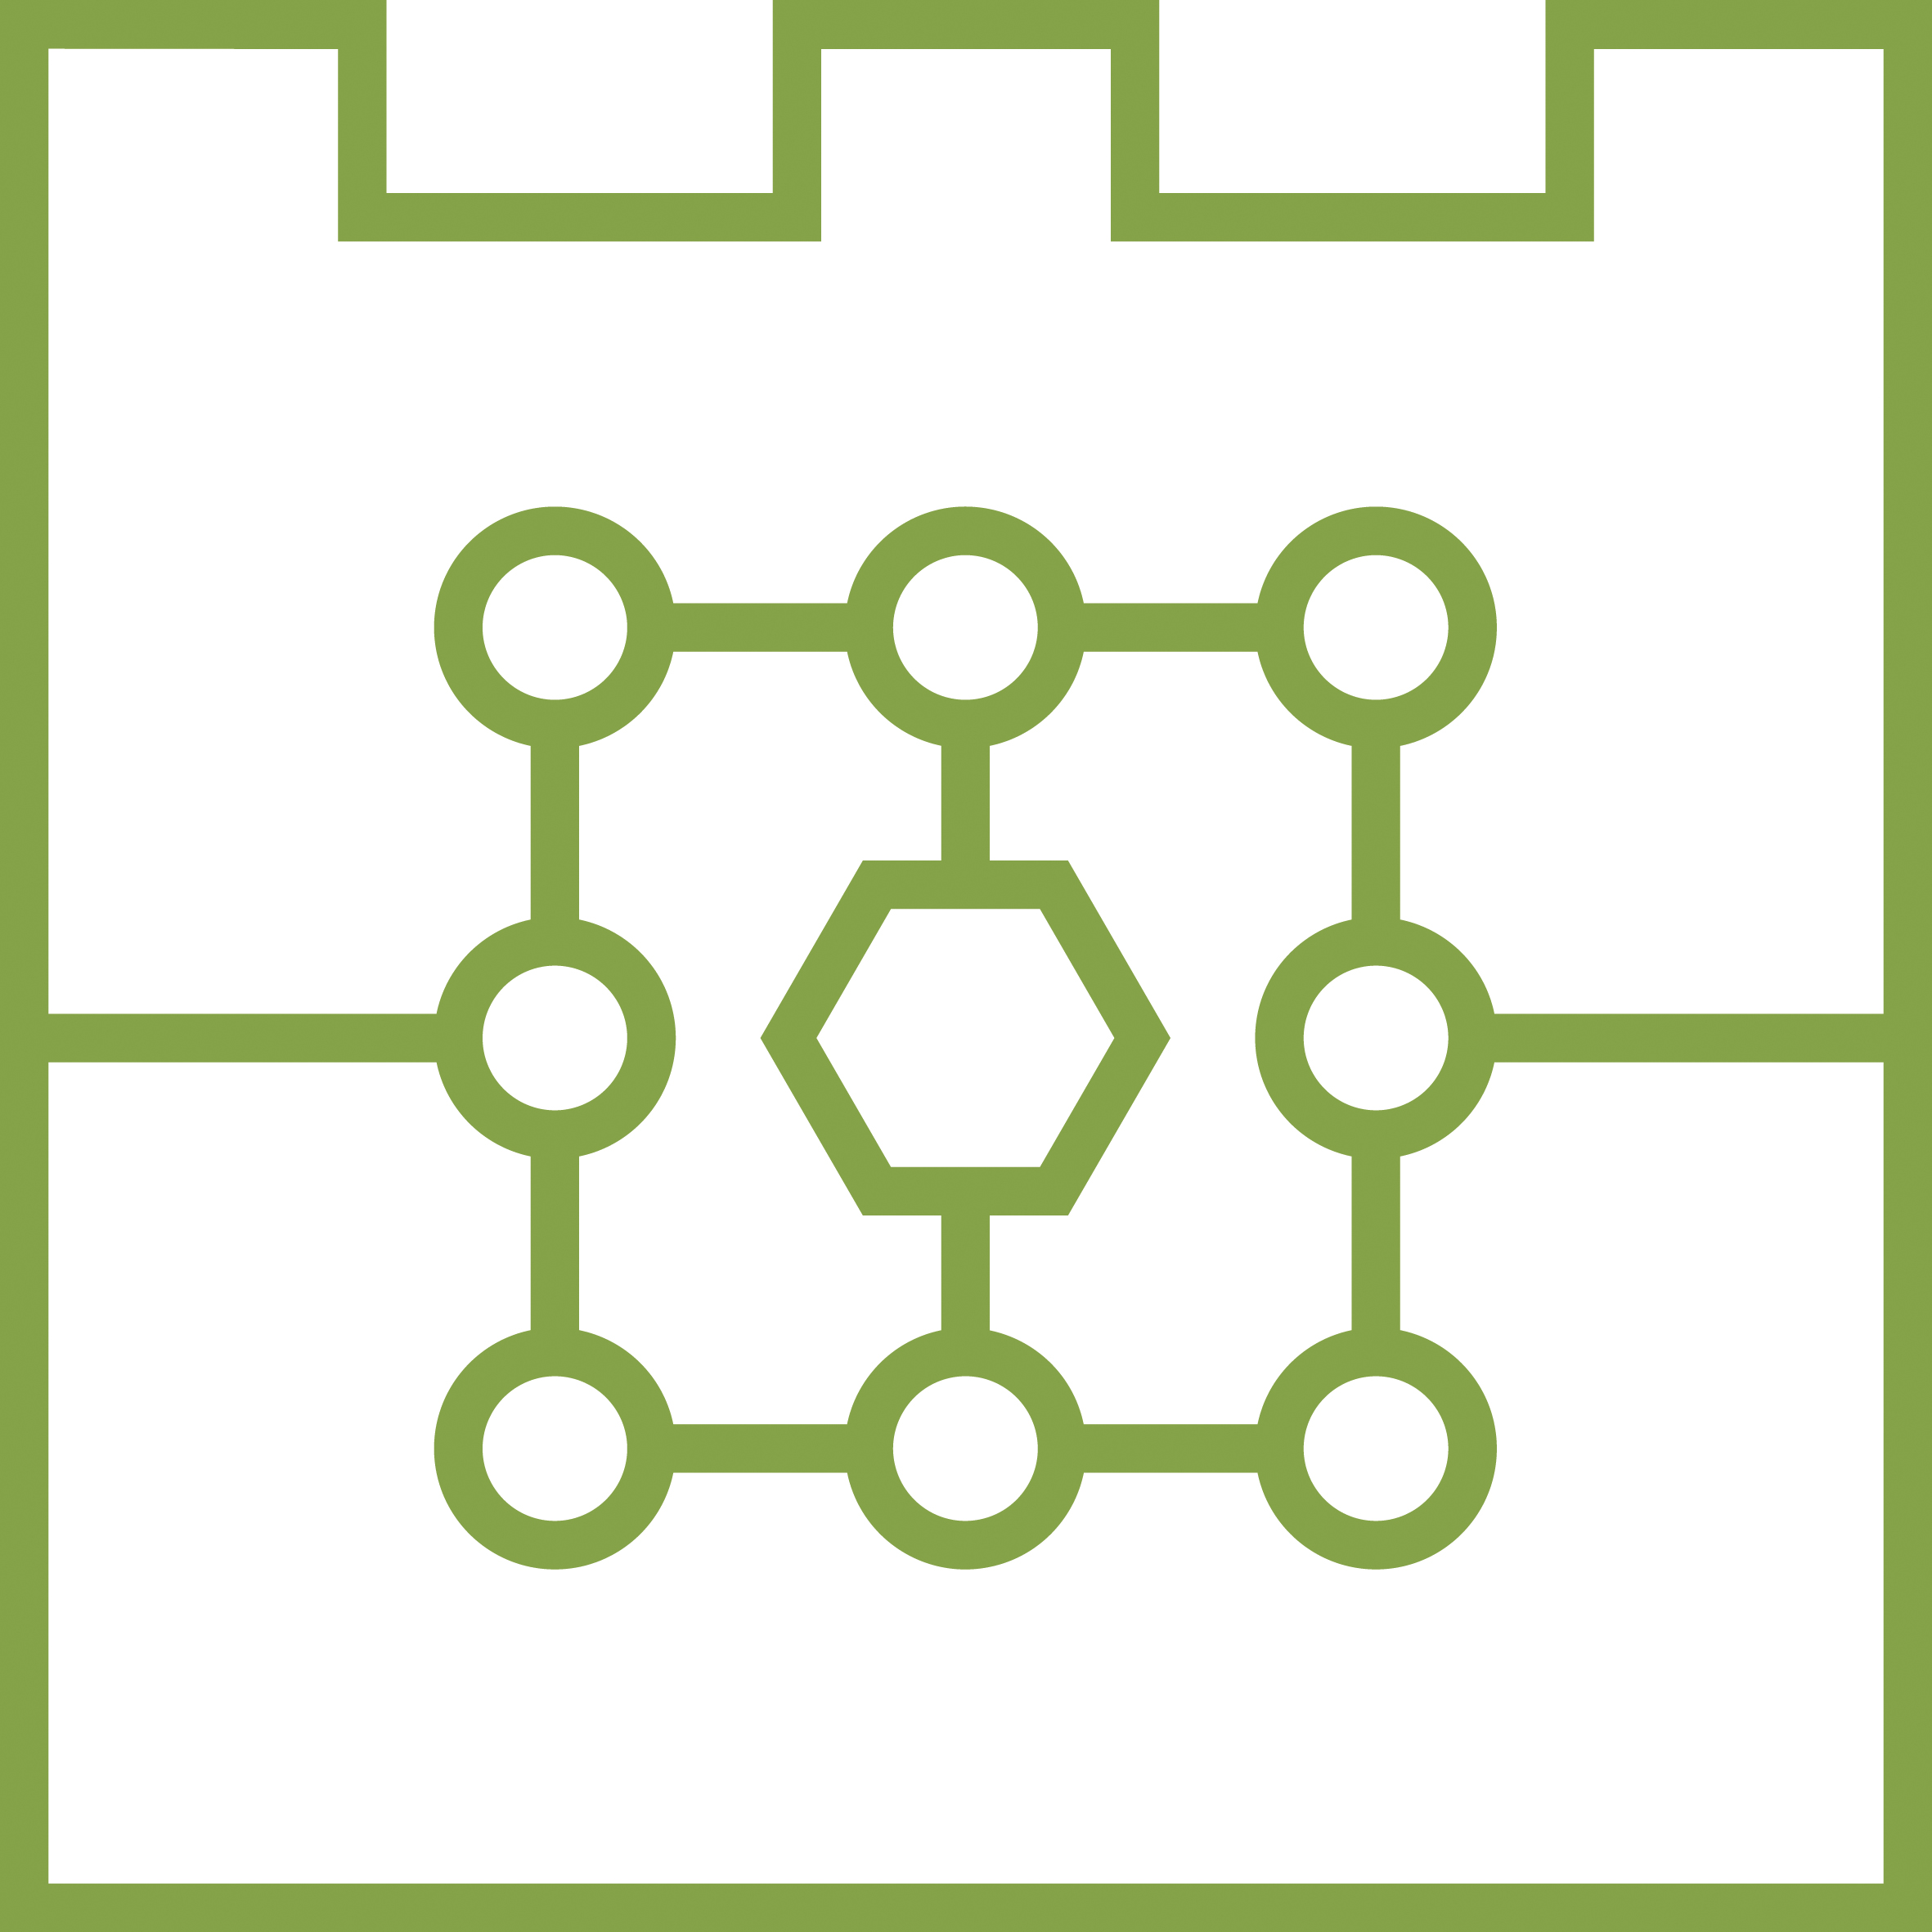
\includegraphics[width=\linewidth]{gfx/LOGO_FACULTY} \\ 
  \end{minipage}

  \vfill
  \vfill

  \begin{center}
    \Large \textbf{\myName}\\
    \vspace{0.3cm}
    \Large \textbf{Index number: 134088}\\
  \end{center}

  \vfill

  \begin{center}
    \LARGE \textbf{Analiza rozwiązań bazodanowych, na przykładzie klastrów energii}
  \end{center} 
  
  \begin{center}
    \LARGE \textbf{\myTitle}
  \end{center} 
  
  \begin{center}
    \LARGE \textbf{B.S. thesis on the Computer Science major}
  \end{center}
  
  \vfill
  
  \hspace{0.6\textwidth} 
  \begin{minipage}{0.4\textwidth}
  Supervisor: \\
  \textbf{\myProf} \\

  Reviewer: \\
  \textbf{dr. Barbara Borowik}
  \end{minipage}

  \vfill
  \vfill
  
  \begin{center}
    Kraków 2023
  \end{center}

\end{titlepage}

\include{frontbackmatter/Titleback}
%\cleardoublepage\include{frontbackmatter/Dedication}
%\cleardoublepage\include{frontbackmatter/Foreword}
%\cleardoublepage\include{frontbackmatter/Declaration}
\condLOCK{\cleardoublepage\include{frontbackmatter/BlockingNotice}}
\cleardoublepage%*******************************************************
% Abstract in English
%*******************************************************
\pdfbookmark[0]{Abstract}{Abstract}


\begin{otherlanguage}{american}
	\chapter*{Abstract}
	
	
\end{otherlanguage}
%\cleardoublepage\include{frontbackmatter/Publications}
%\cleardoublepage\include{frontbackmatter/Acknowledgments}
%\cleardoublepage\include{frontbackmatter/Contents}
%\cleardoublepage\include{frontbackmatter/Figures}
%\cleardoublepage\include{frontbackmatter/Tables}
%\cleardoublepage\include{frontbackmatter/Listings}
\cleardoublepage%*******************************************************
% Acronyms
%*******************************************************
\automark[section]{chapter}
\renewcommand{\chaptermark}[1]{\markboth{\spacedlowsmallcaps{#1}}{\spacedlowsmallcaps{#1}}}
\renewcommand{\sectionmark}[1]{\markright{\thesection\enspace\spacedlowsmallcaps{#1}}}
\refstepcounter{dummy}
\pdfbookmark[0]{Abk\"{u}rzungsverzeichnis}{abkuerzungsverzeichnis}
\markboth{\spacedlowsmallcaps{Abk\"{u}rzungsverzeichnis}}{\spacedlowsmallcaps{Abk\"{u}rzungsverzeichnis}}
\chapter*{Acronyms}

% Insert your acronyms here
\begin{acronym}[UML]
  %\acro{DRY}{Don't Repeat Yourself}
  \acro{DBMS}{Database Managment System}
  \acro{SQL}{Structured Querry Language}
\end{acronym}

\cleardoublepage

%*************************************************************************
% Mainmatter
%*************************************************************************
\cleardoublepage
\pagestyle{scrheadings}
\pagenumbering{arabic}
% Alwas use \cleardoublepage before \part{...}.
\cleardoublepage
\part{Thesis}\label{pt:thesis}
\chapter{Introduction}
\label{ch:intro}
PLACEHOLDER

%
% Section: Motivation
%
\section{Motivation}
\label{sec:intro:motivation}
The need to store different kinds and amounts of data, spawned many alternatives to the traditional SQL-based relational Database Management Systems. In such a varied market, the decision as to which Database System to use becomes increasingly difficult and unclear. 
%
% Section: Ziele
%
\section{Goal}
\label{sec:intro:goal}
This thesis will choose the best database solution for the data processing and storage needs of an energy cluster, based on carefully analyzing different DBMSs avialable on the market.

%
% Section: Struktur der Arbeit
%
%\section{Structure}
%\label{sec:intro:structure}


\chapter{Database Solutions}
\label{ch:background}
\par There are numerous distinct database solutions avialabe on the market already, each boasting their own unique characteristics and design philosophy. Generally database engines are divided into two categories:
\begin{description}
  \item[SQL databases] based on a relational model, their engines implement some dialect of the SQL language.
  \item[NoSQL databases] a term used to describe various other database solutions, that rely on documents, graphs, key-value pairs or other structures to organize their data, rather than the relational model endorsed by SQL.
\end{description}

\par Generally, the latter compromise consistency of data in favor of data avalibility and speed of data processing.

%
\section{SQL}
\label{sec:background:first_section}
\par Structured Query Language (SQL) is a collection of various languages used to define interaction between the user and the database engine. Initially developed in the 70s at IBM, it gained quick popularity and dominated the Relation Database Management System market.\citep{SQLHandbook} 
\par The relational database organazation model, used in SQL organizes data into two-dimensional array structures called tables. Each table is a series of row-like records of simple data types such as an integer, a string of text or a date, although holding binary data of any kind is possible. These records must all contain the same kind of data, arranged in the same order - the word columns or fields is often used to describe single pieces of data stored in this order. Same data in different tables may be related, and thus create links between these tables, called relations.
\par As it was mentioned earlier, the Structured Query Language is in fact composed of four different languages, each describing different kinds of interactions possible with the Database engine\citep{KreibchSQLite}:
\begin{description}
  \item[SQL Data Manipulation Language] is used to create and modify data.
  \item[SQL Data Definition Language] is used to create and modify structures in which data is stored.
  \item[SQL Data Control Language] is used to grant permission to access and modify data inside the database system.
  \item[SQL Data Query Language] is used to read data from the system in various ways.
\end{description}
\par These languages combined together can create complex queries that can store and access data in various unique ways, satisfying the need of even the most complex database systems.
\par Another important mechanism introduced in SQL is the so called "transaction". It is defined as a set of database queries, executed one after another, whose results are only implemented if all of these queries execute succesfully[SQLHANDBOOK]. These transactions should obey the principles of ACID - Atomicity, Consistency, Isolation, Durability. [ACID]
\begin{description}
  \item[Atomicity] means that if one of the queries that make up a transaction fails, none of the changes implemented by the rest of the transaction takes place.
  \item[Consistency] ensures that wether or not the transaction suceedes, the database will remain in a valid and operational state.
  \item[Isolation] of transactions, requires the data of the inbetween states of a database transaction to be completely invisble and unavialable to other transactions.
  \item[Durability] in terms of transactions, means that after a transaction is sucessfully executed, its effect will stay in the database, even if subsequent operations fail.
\end{description}
\par Implementation of these properties ensures stability and consistency, often required in many database instances. The payoff, however, is the increased amount of computation needed to perform basic operations, since every operation needs to perform certain checks and data analyses in order to conform to these principles.

%
\subsection{SQLite}
\label{subsec:background:first_seciton:first_subsection}
\par In comparison with the rest of SQL based solutions, SQLite is a very unique one, in that it doesn't come with its own engine that is constantly running and waiting for users to connect and issue queries. Rather than that, SQLite stores its data in a simple file stored on a hard drive, that can then be accessed by various SQLite compatible applications that can open, read and modify the file according to the SQL standard, and then close the file.

\par Because of its quirks, SQLite lacks in speed of both reading and writing the data. It also allows only one application to access and modify its databases contents. Its strength however, lies in its lightness, simplicity and low resource intensivity. It acts as an excellent data storage solution for simple apps, especially on mobile devices since they can rarely afford an online only database or constant access to a database hosted on a remote network. It can also find a great deal of use in databases that act as buffers or temporary storage for other, larger systems.\citep{OwensSQLite}

\subsection{PostgresSQL}
\label{subsec:background:first_section:second_subsection}
\par PostgresSQL is one of the most popular open-source implementations of the SQL paradigm \citep{worsleyPostgresSQL}. It also includes its own programming language, PL/pgSQL, used to create advanced procedures as well as to include external scripts from other languages usually not asociated with relational databases, such as Perl or Python. 

\par PostgresSQL expands on the standard relational model of the SQL language, by introducting the concept of objects, inheritance and arrays, known from conventional programming languages. The user can now store multiple values in a single column, create child-parent relationships between tables and even create complex programs that can be invoked by SQL statements. In this so called object-relational model, tables are sometimes called objects, and columns are sometimes called properties of said objects [ACID].

\section{NoSQL}
\label{sec:background:second_section}
\par As relational databases slowly developed to dominate the DBMS market, their flaws became more apparent. They are relatively easy to use and maintain, and the various languages that comprise the SQL standard allow execution of as simple or as complex operations as the user needs. 
\par The above mentioned transaction mechanism and their ACIDidty takes care of the heavy lifting required to ensure stability of extensive database systems. This very same ACIDity however, takes its toll on the performance of the DBMS, since every operation needs to be completed ensuring every single one of the ACID principles are complied with. This problem becomes especially exacerbated, when dealing with distributed database implementations, present concurently on multiple systems [CASSANDRA]. To deal with this problem, a special protocol called \textbf{"two-phase commit protocol"} was invented. When using this protocol, a special coordinator mediates between the user and every system that the database consists of. It first sends the query to every DBMS participating in the distributed network, waits until every single one of these participants finishes to execute the transaction up until the very last step where the transaction is "commited" to the database (hence the name). If every single one of these members executes the transaction successfully, it sends a all clear signal to every subsystem and allows them to finalize the transaction, if anything goes wrong in either system, the coordinator ensures that the transaction is canceled everywhere [2PC]. Unfortunetaly, since this 2PC locks every resource the transaction uses and extends the time needed to complete an operation, it is only really useful in tiny operations that can complete very quickly without compromising the responsiveness of the entire system, which is not always the case and is one of the reasons why you may not always want to ensure the ACIDity of every single operation [CASSANDRA].
\par Another problem with RDBMS is the traditional structure of SQL based database schemas. They require the user to store data in rigid tables, that often necessitate the use of special tables representing various relationships such as one-to-many, many-to-many or one-to-one. This model only makes complex queries even harder to compose and interpret by a human, and makes complex database schemas especially difficult to read. Also, in many cases it is extremely challenging to design a database schema that acurately represents the necessary data, while complying with the RDBMS model [CASSANDRA].
\par In summary, while excellent in many general cases, certain DBMS implementations may require to go beyond the constraints of the SQL model. These SQL-defying database solutions began to be called NoSQL or "Not only SQL" [SQLvNOSQL].

\subsection{Cassandra}
\label{subsec:background:second_section:first_subsection}
\begin{center}
''Apache Cassandra is an open source, distributed, decentralized, elastically scalable, highly available, fault-tolerant, tuneably consistent, row-oriented database that bases its distribution design on Amazon's Dynamo and its data model on Google's Bigtable. Created at Facebook, it is now used at some of the most popular sites on the Web''
\par - Cassandra: The Definitive Guide: Distributed Data at Web Scale, Jeff Carpenter, Eben Hewitt
\end{center}

\subsection{MongoDB}
\label{subsec:background:second_section:second_subsection}
\par MongoDB is an excellent example of the NoSQL database design paradigm, moving away from the relational database model, in favor of document-oriented one \citep{mongoDB}. Instead of rows, MongoDB introduces documents - loose collections of data representant of how modern object-oriented programmers organize their data. MongoDB databases are much more flexible and easier to add data to and expirement in, thanks to MongoDB not requiring a fixed schema for all documents inside of one data collection.
%
\par MongoDB is also excellent for large databases that often have to be spread across several machines to be scaleable - the MongoDB engine automatically handles balancing documents across various machines in a single cluster. 

\par MongoDB documents are ordered sets of key-value pairs, simmilar to dictionaries or maps known from conventional programming languages. These documents are represented using the JSON standard, making them very intuitive to expirenced programmers. These documents are grouped in collections, analogous to SQL's tables. 

\par MongoDB's interface is a fully featured javascript interpreter, giving the user the flexibility of the entire JS language complete with its standard libraries. Queries, inserts, deletions and modifications to the data can be done via MongoDB's javascript compatible API.

\subsection{Prometheus}
\label{subsec:background:second_section:thrid_subsection}
\par Prometheus is an implementation of another famous NoSQL approach - the time series database. It specificaly collects data as a series of key/value pairs and timestamps representing the time data was gathered. Usually this data, often called samples, is collected periodically from the same source. 
\par Time series databases are an excellent way to store large amounts of data in a very short period of time, they store data very efficiently and help save calculation costs.

\chapter{Demands of an Energy Cluster}
\label{ch:background}
\par An \textbf{Energy Cluster} is a group of institutions, businesses, and individual customers working to produce, exchange, and distribute electrical energy. These clusters allow smaller agents in the energy market to cooperate and pool their resources to make their energy infrastructure safer, more efficient, and more profitable. This arrangement allows these entities to get more favorable deals when buying and selling electricity back to the grid \citep{UwarunkowaniaRozwojuEnergetykiRozproszonej}. 
\par Energy clusters typically include mid-sized enterprises and smaller individual energy plants, but they can also include larger institutions dedicated solely to generating electricity. 
\par Energy clusters also help to promote the development of renewable energy sources, such as solar, wind, and hydroelectric \citep{UwarunkowaniaRozwojuEnergetykiRozproszonej}.

\section{Historical and legal background} 

\par Fossil fuels, mainly coal, play a crucial role in Polish energy production. Most energy-producing coal plants were built in the waning decades of the previous century. Since then, renewable energy has been on the constant rise, especially solar technologies, which saw a sudden growth in 2020 thanks to the influx of prosumers - entities simultaneously producing and consuming energy \citep{CarbonPoland} \citep{Prosumer}.
\par Five large governmental entities dominate the Polish energy distribution market, each operating in its distribution area. These large distribution network operators (or DNO) are, in order of their size \citep{dostawcyPradu}:
\begin{itemize}
  \item Tauron Dystrybucja S.A.
  \item PGE Dystrybucja S.A.
  \item ENERGA-OPERATOR SA.
  \item Enea S.A.
  \item E.ON Polska S.A. (formerly innogy Polska S.A.)
\end{itemize}
\begin{figure}[htbp]
 \centering
 
\includegraphics[width=0.5\textwidth]{gfx/EnergyDistributionMap}
 \caption{Distribution Network Operators in Poland \citep{mapkaEprad}}
 \label{fig:chapter02:energydistribution}
\end{figure}
\par Energy Clusters introduce a local alternative to these large enterprises. 
\par The Polish Law defines an energy cluster as ''Cywilnoprawne porozumienie, w skład którego mogą wchodzić osoby fizyczne, osoby prawne, jednostki naukowe, instytuty badawcze lub jednostki samorządu terytorialnego, dotyczące wytwarzania i równoważenia zapotrzebowania, dystrybucji lub obrotu energią z odnawialnych źródeł energii lub z innych źródeł lub paliw, w ramach sieci dystrybucyjnej o napięciu znamionowym niższym niż 110 kV, na obszarze działania tego klastra nieprzekraczającym granic jednego powiatu lub 5 gmin. Obszar działania klastra energii ustala się na podstawie miejsc przyłączenia wytwórców i odbiorców energii będących członkami tego klastra.'' [A Civil law agreement, between natural persons, legal persons, research institutions or local governments, on production, exchange, distribution or turnover of energy from renewable energy sources, or other sources or fuels, as a part of a distribution network with rated voltage lower than 110 kV, and an operational area lower than one county or five municipalities. The energy cluster's operational area is defined, based on the locations of energy producers and consumers, belonging to that energy cluster.]  (art. 2 p. 15a Act on Renewable Energy Sources) \citep{RESAct}.
\par These Energy clusters are represented by an Energy Cluster Coordinator, defined by polish law as ''Spółdzielnia, stowarzyszenie, fundacja, wskazane w porozumieniu cywilnoprawnym lub dowolny członek klastra energii, powołany w celu reprezentowania klastra'' [A cooperative, assocation, foundation, mentioned by a civil law agreement, or any energy cluster member, obligated to represent the cluster] (art. 2 p. 15a Act on Renewable Energy Sources)\citep{RESAct}.
\par Energy clusters are thus not an entity onto themself but an accord that defines its participants, operational area, its representative in the form of the coordinator, and its purpose and activities, whether that be production, distribution, sale, or storage of energy. It should also define the rights and responsibilities of every cluster member, the internal organization of the cluster, and how the agreement may be altered or dissolved \citep{erKlaster}.
\par One common type of an energy cluster member is the so-called prosumer, a portmanteau of producer and consumer. The RES act defines them as entities buying and producing energy from renewable sources for their own purposes \citep{Prosumer} \citep{RESAct}. 

\section{The functioning of energy clusters}

\par To establish a functioning energy cluster, its members should define a name and location of the cluster, list all of its members, and name one of them the coordinator, whose role is to manage the cluster and ensure work inside it goes smoothly \citep{erKlaster}.
\par The most apparent duty of energy clusters is to produce, exchange, and sometimes store electricity their members produce or buy from the outside grid. The necessary infrastructure can be either borrowed from the public grid upon a prior agreement or be explicitly built for the cluster.
\par Another essential responsibility of every cluster member is to measure how much energy each produces and consumes, along with the quality of said energy. These measurements are then analyzed to ensure compliance with the cluster agreement and national energy production and distribution laws \citep{erKlaster}.
\par The energy produced by clusters usually comes from renewable sources, although current law also allows some use of fossil fuels \citep{UwarunkowaniaRozwojuEnergetykiRozproszonej}.

\section{The Energy Cluster infrastructure}

\par The energy cluster members need to agree on the energy delivery method. These entities can exchange energy by using: 
\begin{enumerate}
  \item existing infrastructure,
  \item their private infrastructure, 
  \item a hybrid model consisting of the previous options.
\end{enumerate}
\par The most economical and popular option is to use the public energy grid. In such cases, the energy cluster coordinator has to apply with the appropriate DNO for access to the infrastructure, and the DNO is obligated to, whenever possible, connect every applying entity to the existing grid without prioritizing any other entity.
\par The less common option is to use a private energy grid explicitly made for the energy cluster. This method comes with responsibilities similar to those imposed on more traditional entities outside the energy cluster and much higher costs than using the public grid. It can, however, be economically sound in the case of many huge energy producers and consumers close to one another.

\section {Members of an energy cluster}

\par Various entities compose an energy cluster, some of which produce or consume energy, and others handle organizational matters. 
\par The public administration is frequently an initiator of such initiatives, especially given their benefits to the local economy and government funding provided for energy cluster development. It may help resolve conflicts of interests of competing cluster members or help procure necessary funding faster and more efficiently \citep {ksiazka}.
\par Some of the most vital members of energy clusters are local businesses. Their membership is mutually beneficial since while energy clusters can help their development, such enterprises provide the necessary funding and experience to build the clusters network faster.
\par The rest of the cluster membership constitutes prosumers with small energy-producing installations capable of satisfying at least some of their energy consumption \citep{erKlaster}.
\par Every energy cluster needs to choose, amongst its members, a coordinator to represent the cluster. It is usually a private company operating in the energy distribution market with the necessary funds and permits to produce and distribute energy. It can apply for any further permits needed in the future and take loans in the name of the cluster. Sometimes, that company acts exclusively as an energy cluster coordinator, efficiently managing the entire system \citep{erKlaster}.
\par The coordinator can also be an association of natural persons making up the energy cluster, a foundation comprising both natural and legal persons, a cooperative, or a company. It has to be a legal person, meaning entities such as partnerships or homeowner associations cannot in themselves be a part of an energy cluster \citep{erKlaster}.

\section{Energy meters}

\par Members of an Energy Cluster must measure power consumption and production in order to reconcile with it. Furthermore, energy meters can also acquire information on energy quality, and compliance with previously established norms. Data gathered by these meters is then used to improve efficiency, reduce costs, and optimize energy usage. They must be installed in every energy cluster member, whether a small prosumer or big industrial plant.
\par One example of an energy meter applicable in energy clusters and available on the market is the Otus 3 Three-phase electricity meter. Designed for residential use and capable of connecting to intelligent systems, it can gather and send to a database essential data about energy quality and its use by an energy cluster member \citep{otus}.
\par Otus 3's creators, the company Apator, in collaboration with Atende Industries, is in the process of creating an improved smart meter, specifically for the purposes of Energy Clusters and decentralized energy \citep{atende}.
\par Some of the most essential parameters gathered or checked against by meters such as Otus 3 include:
\begin{description}
  \item[The total energy produced/consumed] by energy cluster members is essential to monitor for two reasons: calculating an energy-produced-to-consumed balance that compares how much more or less energy was produced than consumed at any given window of time. Since excess energy is delivered to the energy cluster infrastructure to be consumed by other members or sold on the energy market, this balance has to be included in the energy settlement. Another reason to observe the total consumed energy is to monitor the exceedance of \textbf{contracted energy}. Contracted energy is the maximum amount of electrical energy an energy cluster member can consume at any given time. It should be specified in the energy cluster agreement based on the particular member's energy needs and the cluster's infrastructure capacity to provide said energy. Establishing a contracted amount of energy consumption with energy cluster members is a vital step in estimating the capacity of the cluster to satisfy all its members' needs. 
  \item[Reactive power] is the natural consequence of capacitance and inductance's presence in AC systems. When connected to an AC circuit, capacitors and inductors cause a phase shift between the voltage and current in the circuit. A phase shift in the form of reactive power, introduced to the grid, can cause instability and loads of other problems and thus is undesirable. Because capacitors cause a leading phase shift, while inductors cause a lagging one, these shifts can balance each other out; thus, maintaining a proper balance between capacitor-heavy and inductor-heavy devices is essential. A vector on the complex plane can be drawn, with real power drawn on the vertical axis and reactive power drawn on the horizontal axis. Such a vector in systems with leading reactive energy usually lands in the first quadrant of the plane, while lagging reactive energy usually results in the vector landing in the fourth quarter. An entity producing too much reactive energy in either direction has to pay fines per the energy cluster agreement. According to the decree of the Minister of Economy from 18th September 2011, the formula used to calculate the fine paid for excessive reactive energy produced is as follows \citep{psr}: $O_{b} = k \times C_{rk} \times (\sqrt{{{1 + tg^2 \varphi} \over {1 + tg^2 \varphi_{0}}} - 1}) \times A$ where:
\begin{itemize}
  \item $O_{b}$ is the fine paid for excessive reactive energy.
  \item $C_{rk}$ is the price of electrical energy, referred to in Article 23, paragraph 2 point 18, letter b of the law in force on the day of tariff approval.
  \item $k$ is the multiple of price $C_{rk}$ established in the tariff.
  \item $tg \varphi_{0}$ is a power factor established according to the decree.
  \item $tg \varphi$ is a power factor resulting from reactive power. It is equal to ${tg \varphi} = {{{\Delta E_{b}} \over A} + tg \varphi_{0}}$ where $\Delta E_{b}$ is the excess reactive energy recorded by a measuring device within the settlement period.
  \item $A$ is the active energy taken around the clock or for the time zone in which reactive energy consumption is controlled.
\end{itemize}
  \item[Frequency] is the number of cycles per second in an alternating current system, measured in hertz. It is vital to measure it since if the frequency of the electrical energy in an energy grid deviates significantly from the standard frequency, it can cause problems with the equipment connected to the grid, such as equipment operating too fast or causing significant wear. The energy grid operator has to ensure that frequency stays stable according to norms. An entity may monitor frequency to document cases of that duty not being fulfilled. According to the Power System Regulation, ''wartość średnia częstotliwości mierzonej przez 10 sekund w miejscach przyłączenia powinna być zawarta w przedziale: a) 50 Hz ± 1 \% (od 49,5 Hz do 50,5 Hz) przez 99,5\% tygodnia, b) 50 Hz + 4\% / -6\% (od 47 Hz do 52 Hz) przez 100\% tygodnia;'' [the average value of frequency measured in a period of 10 seconds in the point should be within the range of: a) 50 Hz ± 1 \% (from 49,5 Hz to 50,5 Hz) within 99,5\% of a week, b) 50 Hz + 4\% / -6\% (from 47 Hz to 52 Hz) within 100\% of a week] (Power System Regulation)\citep{psr}.
  \item[Voltage] is the difference in electric potential between any two given points. It is another vital qualitative measure of electricity. Similarly to frequency, irregular voltage can slow down or even damage equipment and infrastructure, so it is vital to quickly monitor voltage to fix anomalies. The Power System Regulation Act, prescribes the following limits on allowed voltage: ''w każdym tygodniu 95\% ze zbioru 10-minutowych średnich wartości skutecznych napięcia zasilającego powinno mieścić się w przedziale odchyleń: a) ±10\% napięcia znamianowoego dla sieci o napięciu znamionowym 110V i 220V, b) +10\% / -10\% napięcia znamionowego dla sieci o napięciu znamionowym 400kV'' [within each week, 95\% of the sets of effective values of data gathered over 10 minutes, should be within the range of: a) ±10\% of rated voltage for an energy grid with rated voltage of 110V and 220V, b) +10\% / -10\% of rated voltage for an energy grid with rated voltage of 400kV] (Power System Regulation)\citep{psr}.
\end{description}

\section{Data structure}

\par Data gathered from meters is usually structured as pairs of data values and the time of measurement timestamps. Additional information, such as data acquisition to the database timestamp or the data's point of origin, may also be included, depending on the implementation. 
\par A sample series of data gathered from a particular energy meter over the year 2022 has been provided by the Energy Cluster in Ochotnica Dolna. Data in this set is first organized into separate metrics, described by rows of data, each containing\citep{ochotnica}:
\begin{enumerate}
  \item A timestamp, representing the time and date of data capture.
  \item A timestamp, representing the time and date of data acquisition into the database.
  \item A real number, representing the metric's value at the given point in time.
  \item An integer, representing an ID of the energy meter that provided the data.
\end{enumerate}

\begin{table}[!ht]
    \centering
    \caption{Energy consumed at one member of the Energy Cluster in Ochotnica Dolna \citep{ochotnica}}
    \begin{tabular}{llll}
    \hline
        "cap\_time (utc)" & "acq\_time (utc)" & "value" & "origin" \\ \hline
        "2021-09-14 10:30:00,000" & "2021-09-21 09:05:59,004" & "0.220" & 1 \\ 
        "2021-09-14 10:45:00,000" & "2021-09-21 09:05:59,472" & "1.804" & 1 \\ 
        "2021-09-14 11:00:00,000" & "2021-09-21 09:05:59,882" & "3.290" & 1 \\ 
        "2021-09-14 11:15:00,000" & "2021-09-21 09:06:00,406" & "4.654" & 1 \\ 
        "2021-09-14 11:30:00,000" & "2021-09-21 09:06:00,921" & "6.143" & 1 \\ 
        "2021-09-14 11:45:00,000" & "2021-09-21 09:06:01,346" & "7.667" & 1 \\ 
        "2021-09-14 12:00:00,000" & "2021-09-21 09:06:01,860" & "9.323" & 1 \\ 
        "2021-09-14 12:15:00,000" & "2021-09-21 09:06:02,284" & "10.817" & 1 \\ 
        "2021-09-14 12:30:00,000" & "2021-09-21 09:06:02,733" & "12.518" & 1 \\ 
        "2021-09-14 12:45:00,000" & "2021-09-21 09:06:03,144" & "14.196" & 1 \\ \hline
    \end{tabular}
\end{table}

\begin{table}[!ht]
    \centering
    \caption{Phase L1 voltage measured at one member of the Energy Cluster in Ochotnica Dolna \citep{ochotnica}}
    \begin{tabular}{llll}
    \hline
        "cap\_time (utc)" & "acq\_time (utc)" & "value" & "origin" \\ \hline
        "2021-09-21 09:12:41,000" & "2021-09-21 09:12:42,146" & "233.740" & 1 \\ 
        "2021-09-21 09:13:40,000" & "2021-09-21 09:13:41,992" & "231.355" & 1 \\ 
        "2021-09-21 09:14:40,000" & "2021-09-21 09:14:41,354" & "236.173" & 1 \\ 
        "2021-09-21 09:15:40,000" & "2021-09-21 09:15:41,299" & "229.385" & 1 \\ 
        "2021-09-21 09:16:39,000" & "2021-09-21 09:16:40,542" & "230.810" & 1 \\ 
        "2021-09-21 09:17:40,000" & "2021-09-21 09:17:41,683" & "227.255" & 1 \\ 
        "2021-09-21 09:18:39,000" & "2021-09-21 09:18:41,027" & "227.516" & 1 \\ 
        "2021-09-21 09:19:39,000" & "2021-09-21 09:19:41,054" & "227.345" & 1 \\ 
        "2021-09-21 09:20:39,000" & "2021-09-21 09:20:40,305" & "227.166" & 1 \\ 
        "2021-09-21 09:21:38,000" & "2021-09-21 09:21:39,634" & "232.959" & 1 \\ \hline
    \end{tabular}
\end{table}

\par Metrics captured by said meter include:
\begin{itemize}
  \item Energy provided to the energy grid [kV]
  \item Energy consumed from the energy grid [kV]
  \item Quarter 1 reactive energy [kVAr]
  \item Quarter 2 reactive energy [kVAr]
  \item Quarter 3 reactive energy [kVAr]
  \item Quarter 4 reactive energy [kVAr]
  \item Power line frequency [Hz]
  \item Phase 1 effective value of voltage [V]
  \item Phase 2 effective value of voltage [V]
  \item Phase 3 effective value of voltage [V]
\end{itemize}
\chapter{Proposed solutions}
\label{ch:background}
\chapter{Implementation}
\label{ch:background}
\chapter{Results}
\label{ch:background}
%*************************************************************************
% Recommendations
%*************************************************************************
%\part{Empfehlungen zur Erstellung wissenschaftlicher Abschlussarbeiten}
%\label{pt:recommendations}
%*************************************************************************
% Backmatter
%*************************************************************************
% \appendix
%\renewcommand{\thechapter}{\alph{chapter}}
% \cleardoublepage
% \part{Appendix}
%*************************************************************************
% Other Stuff in the Back
%*************************************************************************
\cleardoublepage\include{frontbackmatter/Bibliography}
%*************************************************************************
% Game Over: Restore, Restart, or Quit?
%*************************************************************************
\end{document}
%*************************************************************************
